\chapter{Codegenerierung für WebAssembly}
\label{cha:Codegenerierung-für-WebAssembly}

Dieses Kapitel befasst sich mit der Generierung von WebAssembly-Bytecode. Dabei wird darauf eingegangen, wie MiniJava-Sprachkonstrukte auf WebAssembly abgebildet werden. Manche Sprachkonstrukte setzen Interaktion mit JavaScript voraus. In diesem Kapitel wird dabei nur die WebAssembly-Seite betrachtet, auf das JavaScript-Gegenstück wird in Kapitel \ref{cha:JavaScript-Integration} eingegangen. Weiters wird in diesem Kapitel auf den Aufbau der gesamten Implementierung eingegangen. Das Ergebnis der Codegenerierung in diesem Kapitel ist ein WebAssembly-Modul im Arbeitsspeicher. Auf das Schreiben des Moduls in eine Datei, sowie auf weitere erzeugte Dateien wird in Kapitel \ref{cha:JavaScript-Integration} eingegangen.

Beim Generieren von Bytecode wird in diesem Kapitel davon ausgegangen, dass sämtlicher zu kompilierender MiniJava-Quelltext semantisch korrekt ist. Das bedeutet, dass ausschließlich der Schönwetterfall betrachtet wird, in dem zum Beispiel Variablen vor der Verwendung deklariert werden, Variablen nicht doppelt deklariert werden, aufzurufenden Methoden existieren oder verwendete Datentypen in Ausdrücken zu einander kompatibel sind. Auf die Fehlerbehandlung wird nicht eingangen, da dies aufgrund des großen Umfangs an Fehlerfällen den Rahmen sprengen würde und der Fokus dieses Kapitels auf der Codegenerierung liegt, die syntaktisch und semantisch korrekten MiniJava-Quelltext voraussetzt.

Der für ein Sprachkonstrukt generierte Bytecode wird in diesem Kapitel schablonenartig als \emph{Vorlage} gezeigt. Der Bytecode in diesen Vorlagen ist in der textuellen Repräsentation von WebAssembly dargestellt. Darin befinden sich Platzhalter (gekenntzeichnet durch spitze Klammern \lstinline{<...>}), die beispielsweise auf generierten Bytecode anderer Sprachkonstrukte, andere Instruktionen oder Compile-Zeit-Konstanten verweisen. Weiters kann es vorkommen, dass Teile der Vorlage nur in bestimmten Fällen generiert werden. Diese Teile werden durch eckige Klammern \lstinline{[...]} gekennzeichnet.

\section{Gradle-Projektaufbau}

Das Gradle-Projekt besteht aus fünf Gradle-Modulen:
\begin{itemize}
    \item Das Modul \emph{grammar} enthält die Grammatik von MiniJava in Form der ANTLR-Syntax. In der dazugehörigen \emph{build.gradle}-Datei wird die Scanner-, Parser- und Visitorgenerierung mit dem ANTLR-Gradle-Plugin konfiguriert.
    \item Das Modul \emph{compiler} ist für das Abarbeiten des Syntaxbaums verantwortlich und erzeugt daraus ein WebAssembly-Modul.
    \item Das Modul \emph{wasm} enthält Datenstrukturen zum Aufbau eines Web\-As\-sem\-bly-Mo\-duls im Arbeitsspeicher. Der Aufbau und die Namen dieser Datenstrukturen entsprechen der WebAssembly-Spezifikation \cite{WebAssemblySpecification}. Weiters werden Methoden zur Verfügung gestellt, um aus dem WebAssembly-Modul die textuelle Repräsentation und in weiterer Folge auch die binäre Repräsentation des Modules zu erzeugen.
    \item Das Modul \emph{demo-nodejs} enthält ein Beispiel, wie MiniJava in einer Node.js-Kon\-so\-len\-anwendung eingesetzt werden kann. Darauf wird in Abschnitt \ref{sec:NodeJSExample} eingegangen.
    \item Das Modul \emph{demo-browser} enthält eine Web-Anwendung, in der MiniJava eingesetzt wird. Darauf wird in Kapitel \ref{cha:DemoAnwendung} eingegangen.
\end{itemize}

Zusätzlich ist im Gradle-Projekt noch ein Hilfsmodul \emph{buildSrc} enthalten. Dieses ermöglicht, den MiniJava-Compiler in Gradle-Modulen zu verwenden. Darauf wird in Abschnitt \ref{sec:GradleTask-und-Plugin} eingegangen.

Neben den Gradle-Modulen ist noch eine Standardbibliothek für MiniJava im Verzeichnis \emph{stdlib} enthalten. Datails dazu finden sich in Abschnitt \ref{sec:Standardbibliothek}.

Weiters wird das Node.js-Skrip \emph{run.js} zur Verfügung gestellt, mit dem Erzeugnisse des MiniJava-Compilers direkt ausgeführt werden können, ohne sie in eine eigene Anwendung integrieren zu müssen.

\section{Symboltabellen}

Im Laufe der Codegenerierungen werden sämtliche Metainformationen aller zu kompilierenden MiniJava-Quelltexte in Symboltabellen verwaltet.

Insgesamt werden dazu sechs Symboltabellen eingesetzt, die teilweise hierarchisch miteinander verbunden sind:
\begin{itemize}
    \item Die \lstinline{ClassSymbolTable} verwaltet die Klassen in MiniJava. Eine Klasse ist über den Namen eindeutig identifizierbar. Der WebAssembly-Funktionsindex des Konstruktors wird in dieser Symboltabelle abgelegt. Weitere Metainformationen der Klasse werden in den nachfolgenden drei Kindsymboltabellen, die für jede Klasse separat angelegt werden, verwaltet:
    \begin{itemize}
        \item Die \lstinline{MethodSymbolTable} verwaltet Methoden innerhalb einer Klasse. Eine Methode ist über den Namen und die Datentypen der Parameter eindeutig identifizierbar. Zu jeder Methode wird der WebAssembly-Funktionsindex, der Typ des Rückgabewerts gespeichert. Weiters wird gespeichert, ob die Methode mit den Schlüsselwörtern \lstinline{native}, \lstinline{public} oder \lstinline{static}  gekennzeichnet wurde.
        \item Die \lstinline{FieldSymbolTable} verwaltet Datenkomponenten einer Klasse. Eine Datenkomponente ist über den Namen eindeutig identifizierbar. Für jede Datenkomponente werden der Datentyp und die WebAssembly-Funktionsindizes des \emph{Getters} und \emph{Setters} gespeichert.
        \item Die \lstinline{InitializerSymbolTable} verwaltet die Initialisierer einer Klasse. Ein Initialisierer ist über die Datentypen der Parameter eindeutig identifizierbar. Für jeden Initialisierer wird der dazugehörige WebAssembly-Funktionsindex gespeichert.
    \end{itemize}
    \item In der \lstinline{StringLiteralSymbolTable} werden alle im MiniJava-Quelltext vorhandenen Zeichnkettenliterale gespeichert, um daraus auf die Referenz der Zeichenkette schließen zu können.
    \item Die \lstinline{LocalVariableSymbolTable} verwaltet lokale Variablen und Parameter innerhalb eines Methoden- oder Initialisiererrumpfs. Lokale Variablen und Parameter sind über den Namen eindeutig identifizierbar, dabei werden verschachtelte Gültigkeitsbereiche mitberücksicht. Für jede lokale Variable bzw. jeden Parameter wird der Datentyp und der WebAssembly-Index gespeichert.
\end{itemize}

Bei einem Compiler-Aufruf werden mehrere MiniJava-Quelltexte gemeinsam kompiliert. Innerhalb dieses Vorgangs wird genau eine \lstinline{ClassSymbolTable}-Instanz für alle MiniJava-Klassen verwendet. Es wird ebenfalls nur eine \lstinline{StringLiteralSymbolTable}-Instanz für alle Zeichenketten-Literale eingesetzt. Beim Codegenerieren jeder Methode bzw. Initialisierers wird eine eigene \lstinline{LocalVariableSymbolTable}-Instanz verwendet, die danach nicht mehr benötigt wird.

\section{Abarbeitung des Syntaxbaums in mehreren Phasen}

Da MiniJava wie Java Vorwärtsreferenzen (zum Beispiel für das Aufrufen einer Methode, die erst weiter unten im Quelltext definiert wird) unterstützen soll, ist es leider nicht möglich, den gesamten Syntaxbaum in einem Durchlauf abzuarbeiten. Daher wird der Syntaxbaum in zwei Phasen abgearbeitet:

\begin{enumerate}
    \item Deklarationsphase: In dieser Phase werden alle Klassennamen, Datenkomponenten, Initialisierer und Methoden gesammelt. Daraus wird die \lstinline{ClassSymbolTable}-Instanz mit den dazugehörigen Kindsymboltabellen aufgebaut. Genauer betrachtet wird innerhalb dieser Phase der Syntaxbaum zwei Mal abgearbeitet: Beim ersten Durchlauf werden die Klassennamen gesammelt, im zweiten Durchlauf die Datenkomponenten, Initialisierer und Methoden. Das hat den Grund, dass Datenkomponenten, Initialisierer und Methoden Vorwärtsreferenzen auf Klassen enthalten könnten, zum Beispiel als Datentyp eines Parameters. Mit Hilfe eines \lstinline{Visitors} können nur die relevanten Teile des Syntaxbaums ausgewertet werden, so wird verhindert, dass zu diesem Zeitpunkt irrelevante Teile, wie beispielsweise einzelne Anweisungen, unnötig abgearbeitet werden.
    \item Codegenerierungsphase: Mit Hilfe der in der ersten Phase gewonnenen Metainformationen kann nun der WebAssembly-Bytecode generiert. In dieser Phase wird der Syntaxbaum genau einmal abgearbeitet. Das Ergebnis dieser Phase ist ein WebAssembly-Modul im Arbeitsspeicher.
\end{enumerate}

\section{Indexräume für Funktionen}

Funktionen sind in einem WebAssembly-Modul über einen Index adressierbar. Einige MiniJava-Sprachkonstrukte, wie beispielsweise Methoden, werden auf WebAssembly-Funktionen abgebildet. Ein Teil dieser Funktionen wird direkt in WebAssembly definiert und für diese werden WebAssembly-Instruktionen generiert. Der andere Teil wird importiert, da die Implementierung der Funktion in JavaScript vorliegt.

Die WebAssembly-Spezifikation sieht folgende Einschränkung zur Reihenfolge der Funktionen vor: Zunächst müssen Funktionen importiert werden, erst dürfen Funktionen (inkl. Instruktionen) definiert werden \cite{WebAssemblySpecification}. Allgemein betrachtet erhalten importierte Funktionen somit den Indexbereich von $0$ bis $n$ und in WebAssembly definierte Funktionen den Indexbereich von $n+1$ bis $m$ 

Unter Berücksichtigung dieser Einschränkung werden die Funktionsindizes in der Deklarationsphase gemäß dem Schema in Tabelle \ref{tab:functionIndices} vergeben. Für nicht-native Methoden und Initialisierer müssen WebAssembly-Instruktionen generiert werden, daher bekommen sie die höchsten Funktionsindizes. Sprachinterne Funktionalitäten für Felder und Zeichenketten (siehe Abschnitt \ref{sec:Sprachinterne-Funktionalitäten}), native Methoden, Konstruktoren, \emph{Getter} und \emph{Setter} erhalten die niedrigeren Indizes.

Die sprachinterenen Funktionalitäten wurden an den Anfang gesetzt, damit die darin enthaltenen Funktionen immer am selben Index erreichbar sind, dies erleichtert die Implementierung.

\begin{table}[]
    \centering
    \begin{tabular}{| r | l |}
        \hline
        $0$ & \multirow{2}{*}{Sprachinterne Funktionalitäten} \\
        $a$ & \\
        \hline
        $a+1$ & \multirow{2}{*}{Native Methoden} \\
        $b$ & \\
        \hline
        $b+1$ & \multirow{2}{*}{Konstruktoren} \\
        $c$ & \\
        \hline
        $c+1$ & \multirow{2}{*}{\emph{Getter} und \emph{Setter}} \\
        $d$ & \\
        \hline \hline
        $d+1$ & \multirow{2}{*}{Nicht-native Methoden} \\
        $e$ & \\
        \hline
        $e+1$ & \multirow{2}{*}{Initialisierer} \\
        $f$ & \\
        \hline
    \end{tabular}
    \caption{Aufteilung der Indizes für die entsprechenden WebAssembly-Funktionen}
    \label{tab:functionIndices}
\end{table}

\section{Codegenerierung für nicht-native Methoden}

Objektmethoden und Klassenmethoden werden auf in WebAssembly definierte Funktionen abgebildet. Dabei wird ein Funktionstyp (\lstinline{(type ...)}) im WebAssembly-Modul definiert, der die Schnittstelle der Funktion beschreibt. Haben mehrere Funktionen diesselbe Schnittstelle, werden Typen wiederverwendet. Jede WebAssembly-Funktion referenziert auf den entsprechenden Typ.

\subsection{\lstinline{this}-Parameter}
\label{subsec:this-Parameter}
Objektmethoden benötigen eine Referenz auf das Objekt selbst. Diese Referenz ist im Methodenrumpf über das Schlüsselwort \lstinline{this} abrufbar. Daher wird für Objektmethoden ein zusätzlichen Parameter definiert, auch \lstinline{this}-Parameter genannt, über den sie die Referenz auf das Objekt zur Laufzeit erhalten können. Der \lstinline{this}-Parameter ist bei Objektmethoden immer der erste Parameter.

\subsection{Rückgabetyp}
Falls in MiniJava ein Rückgabetyp (ungleich \lstinline{void}) für die Methode definiert wurde, muss dieser in der Funktionsdefinition mit \lstinline{(result ...)} angegeben werden. Zusätzlich wird als letzte Instruktion im Funktionsrumpf \lstinline{unreachable} eingefügt, Details dazu folgen im nächsten Abschnitt.

Der generierte Bytecode für die gesamte Methode entspricht der Vorlage in Listing \ref{lst:method-bytecode}. Teile in eckigen Klammern werden nur wenn benötigt generiert.

\lstinputlisting[label = {lst:method-bytecode}, caption = {Vorlage für Objekt- und Klassenmethoden}]{src/webAssemblyCodegenerierung/method.wasm}

\subsection{\lstinline{unreachable}-Instruktion}
Auf den ersten Blick erscheint es nicht nachvollziehbar, warum bei Web\-As\-sem\-bly-Funk\-tio\-nen mit Rückgabetyp am Ende die \lstinline{unreachable}-Instruktion generiert wird, da die Methoden, die einen Rückgabewert liefern, immer über die MiniJava-\lstinline{return}-Anweisung verlassen werden. Die \lstinline{return}-Anweisung wird auf die \lstinline{return}-Instruktion abgebildet.

WebAssembly-Module werden validiert, zum Beispiel beim Einsatz von \lstinline{wat2wasm}. Der Validator kann dabei prüfen, ob vor dem Ausführen der \lstinline{return}-Instruktion immer ein Wert oben am Kellerspeicher liegt. Weiters prüft der Validator, ob am Ende einer Funktion mit Rückgabewert immer ein Wert oben am Kellerspeicher liegt. In gewissen Fällen ist es jedoch möglich, dass eine WebAssembly-Funktion zur Laufzeit immer korrekt ablaufen würde, aber vom Validator als ungültig erkannt wird.

Ein Beispiel für so eine Funktion findet sich in Listing \ref{lst:unreachable-problem}. Die \lstinline{if}-\lstinline{else}-\lstinline{end}-Instruktion liefert immer einen Rückgabewert, egal welcher Zweig ausgeführt wird. Die \lstinline{if}-\lstinline{else}-\lstinline{end}-Instruktion ist allerdings aus WebAssembly-Sicht ein Ausdruck, der selbst einen Wert liefern könnte. Die Instruktion ist vergleichbar zum ternären Operator \lstinline{?:} in Java. Da in diesem Fall die \lstinline{if}-\lstinline{else}-\lstinline{end}-Instruktion keinen Wert liefert, nimmt der WebAssembly-Validator an, dass nach dem Ausführen der \lstinline{if}-\lstinline{else}-\lstinline{end}-Instruktion der Kellerspeicher leer ist und die Funktion keinen Rückgabewert liefern kann.

\lstinputlisting[label = {lst:unreachable-problem}, caption = {Beispiel für eine Funktion, zwar korrekt ausgeführt werden könnte, aber nicht korrekt validierbar ist}]{src/webAssemblyCodegenerierung/unreachableExample.wasm}

In einem GitHub-Issue \cite{WebAssemblyUnreachableWorkaround} wurde dieses Problem diskutiert. Als einfache Lösung für dieses Problem wird vorgeschlagen, die \lstinline{unreachable}-Instruktion am Ende der Funktion hinzuzufügen. Dadurch kommt es aus Sicht des Validators immer zu einem Laufzeitfehler, und die Funktion liefert \emph{nie} einen Rückgabewert, da die Ausführung \emph{abgebrochen wird}.

Der Nachteil bei dieser Vorangehensweise ist, dass man selber dafür sorgen muss, dass alle Zweige der Methode mit der \lstinline{return}-Anweisung verlassen werden, sodass nie das Ende der Funktion erreicht wird, da es sonst tatsächlich zu einem Laufzeit kommt.

\section{Codegenerierung für Initialisierer}

Initialisierer werden auf in WebAssembly definierte Funktionen abgebildet. Wie bei Objektmethoden wird auch hier ein \lstinline{this}-Parameter als erster Parameter verwendet. Weiters wurde festgelegt, dass Initialisierer immer die Referenz auf das Objekt als Rückgabewert liefern müssen. Dies erfolgt automatisch ohne eine explizite Anweisung in MiniJava, daher wird als letzte Instruktion im Initialisierer \lstinline{local.get 0} generiert. Der generierte Bytecode für den gesamten Initialisierer entspricht der Vorlage in Listing \ref{lst:initializer-bytecode}.

\lstinputlisting[label = {lst:initializer-bytecode}, caption = {Vorlage für Initialisierer}]{src/webAssemblyCodegenerierung/initializer.wasm}

\section{Codegenerierung für Ausdrücke}
\label{sec:Codegenerierung-für-Ausdrücke}

\subsection{Abarbeitung des Syntaxbaums}
Der Syntaxbaum wird von einem \lstinline{Visitor} abgearbeitet. Der \lstinline{Visitor} delegiert je nach Ausdruckstyp im Syntaxbaums das Abarbeiten des Ausdrucks an einen eignene Codegenerator. Jeder Codegenerator ist für die Codegenierung eines Teilbereich der Ausdrücke verantwortlich. Diese Aufteilung verbessert die Lesbarkeit und Struktierung des Compilers.

Die Codegenerierung für jeden Ausdruck erfolgt allgemein nach folgendem Prinzip: Jeder Ausdruck im Syntaxbaums wird isoliert in einer eigenen Methode betrachtet. Müssen Kindausdrücke eines Ausdrucks ausgewertet werden, erfolgt dies über die \lstinline{visit}-Methode. Die Kontrolle wird dann \emph{nach unten} an den jeweils verantwortlichen Codegenerator weitergegeben. Durch das Ausführen der \lstinline{visit}-Methode wird Bytecode für das Auswerten des Kindausdrucks erzeugt. Gleichzeitig liefert die \lstinline{visit}-Methode als Rückgabewert den statischen Datentyp des Kindausdrucks, dieser Datentyp wird meist für die weitere Auswertung des eigenen Ausdrucks verwendet. Zum Schluss muss als Rückgabewert der statische Datentyp des eigenen Ausdrucks geliefert werden, damit \emph{höhere} Codegeneratoren damit weiterarbeiten können. Der Ablauf zum Codegenerieren wird in Abbildung \ref{fig:codegenerators} anhand eines einfachen Beispiels dargestellt.

\begin{figure}[]
    \centering
    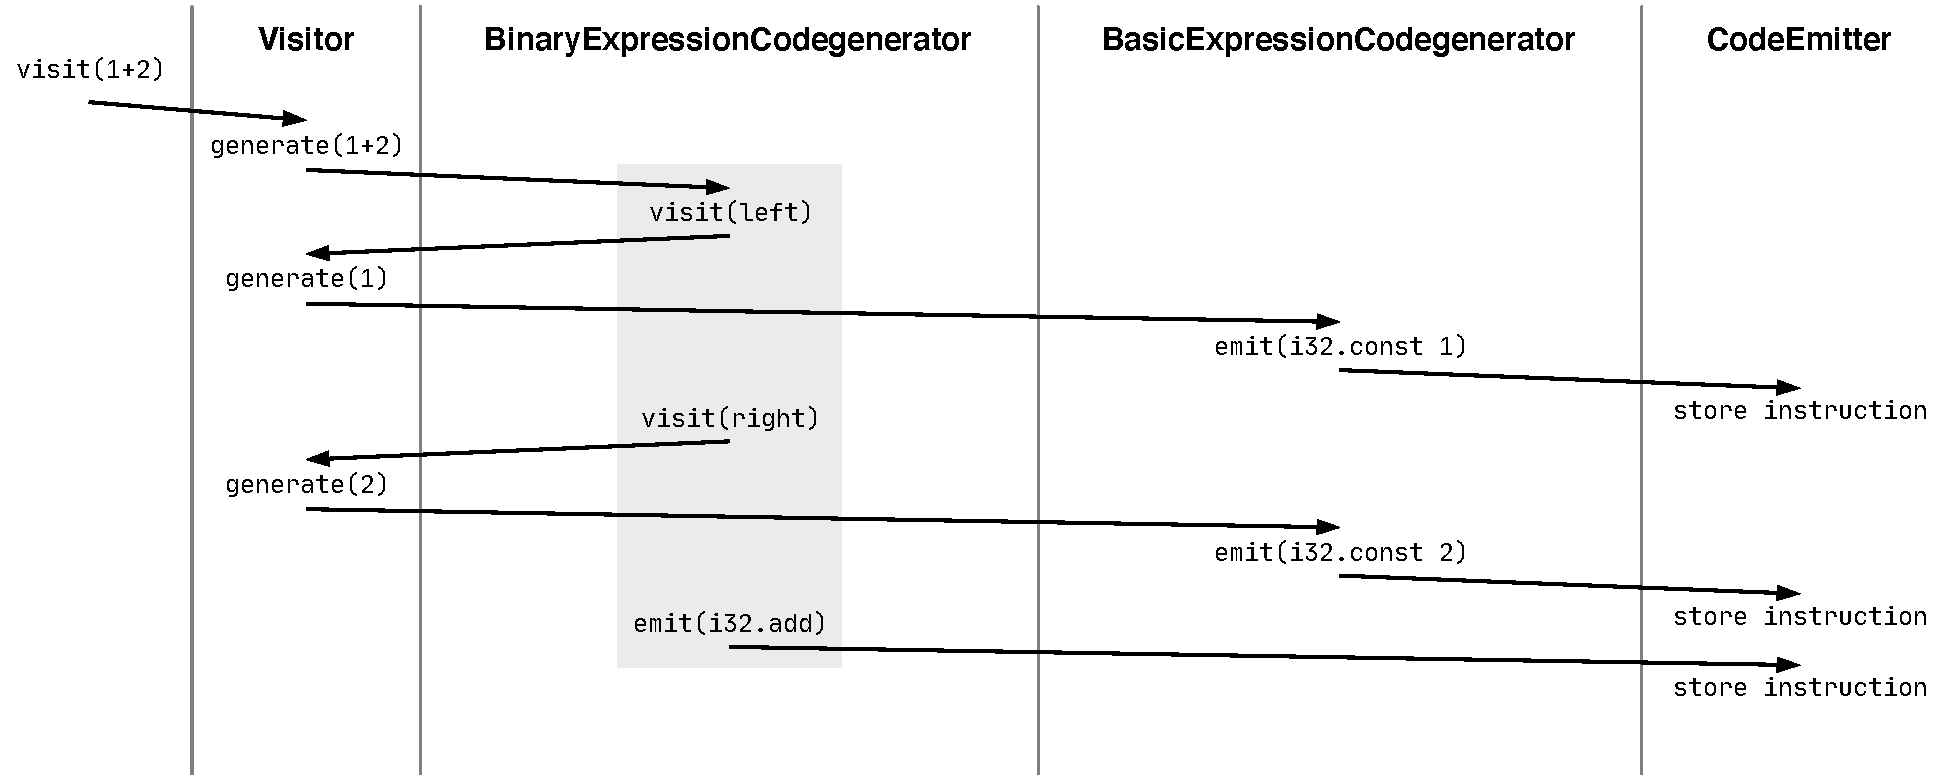
\includegraphics[width=\textwidth]{webAssemblyCodegenerierung/codegenerators}
    \caption{Beispiel für die Codegenerierung des Ausdrucks \lstinline{1+2}. Der Visitor entscheidet anhand der Art des Ausdrucks, welcher Codegenerator verwendet wird. Zunächst wird Code für das Auswerten des linken Teilausdruck ausgewertet, dann Code für den rechten Teilausdruck. Zum Auswerten der Teilausdrücke wird die Kontrolle zurück an den Visitor gegeben. Zum Schluss wird die Instruktion für die Addition direkt generiert.}
    \label{fig:codegenerators}
\end{figure}

In den nachfolgenden Abschnitten wird beschrieben, auf welche Bytecode-Instruktionen Ausdrücke in MiniJava abgebildet werden.

Die Codegenerierung einiger Ausdrücke ist etwas aufwendiger, daher wird in den nachfolgenden Abschnitten nur auf die einfachsten Ausdrücke eingegangen. Den komplexeren Ausdrücken wurden eigene Abschnitte etwas später in diesem Kapitel gewidmet. Zu den komplexeren Ausdrücken zählen: 
\begin{itemize}
    \item Erzeugen von Objekten über den \lstinline{new}-Operator(siehe Abschnitt \ref{sec:Codegenerierung-für-das-Erzeugen-und-Initialisieren-von-Objekten})
    \item Lesen von Datenkomponenten, direkt oder über den Navigationsoperator (siehe Abschnitt \ref{sec:Codegenerierung-für-den-Zugriff-auf-Datenkomponenten})
    \item Erzeugen von Feldern über den \lstinline{new}-Operator (siehe Abschnitt \ref{subsec:Erzeugen-von-Feldern})
    \item Lesezugriff auf Felder über den \lstinline{[]}-Operator (siehe Abschnitt \ref{subsec:Lese-und-Schreibzugriff-mit-Index})
    \item Aufruf von Methoden (siehe Abschnitt \ref{sec:Codegenerierung-für-Methodenaufrufe})
\end{itemize}

\subsection{Schlüsselwort \lstinline{this}}

Das Schlüsselwort \lstinline{this} kann nur in Objektmethoden eingesetzt werden, da die Referenz auf das eigene Objekt über den sogenannten \lstinline{this}-Parameter. Der \lstinline{this}-Parameter ist der erste Parameter in der Parameterliste und gleichzeitig auch die erste lokale Variable in WebAssembly. Das Schlüsselwort \lstinline{this} wird somit durch auslesen dieses Paramters ausgewertet. Dies erfolgt mit der \lstinline{local.get}-Instruktion. Der erzeugte Bytecode entspricht der Vorlage in Listing \ref{lst:this-bytecode}.

\lstinputlisting[label = {lst:this-bytecode}, caption = {Vorlage für das Schlüsselwort \lstinline{this}}]{src/webAssemblyCodegenerierung/this.wasm}

\subsection{Schlüsselwort \lstinline{null}}

Das Schlüsselwort \lstinline{null} steht für eine Referenz, die auf kein Objekt zeigt und wird intern wird auf $0$ abgebildet. Daher wird zur Laufzeit beim Auswerten von \lstinline{null} eine Konstante mit dem Wert $0$ auf den Kellerspeicher mit der \lstinline{i32.const}-Instruktion gelegt.

\lstinputlisting[label = {lst:null-bytecode}, caption = {Vorlage für das Schlüsselwort \lstinline{null}}]{src/webAssemblyCodegenerierung/null.wasm}

\subsection{Literale elementarer Datentypen}

Für alle vier elementare Datentypen können Werte mittels Literale erzeugt werden. Beim Auswerten eines Literals wird zur Laufzeit eine Konstante auf den Kellerspeicher gelegt. Je nach Datentyp erfolgt dies leicht unterschiedlich.

\lstinline{int}-Literale werden auf die \lstinline{i32.const}-Instruktion abgebildet. Die Instruktion erhält als Argument den numerischen Wert des Literals. In der textuellen Repräsentation des Bytecodes wird der Wert als Dezimalzahl-Zeichenkette dargestellt. Der erzeugte Bytecode entspricht der Vorlage in Listing \ref{lst:literalInt-bytecode}.

\lstinputlisting[label = {lst:literalInt-bytecode}, caption = {Vorlage für \lstinline{int}-Literale}]{src/webAssemblyCodegenerierung/literalInt.wasm}

\lstinline{float}-Literale werden auf die \lstinline{f32.const}-Instruktion abgebildet. Die Instruktion erhält als Argument den numerischen Wert des Literals. In der textuellen Repräsentation des Bytecodes wird der Wert als Dezimalzahl-Zeichenkette, mit Dezimalpunkt falls notwendig, dargestellt. Der erzeugte Bytecode entspricht der Vorlage in Listing \ref{lst:literalFloat-bytecode}.

\lstinputlisting[label = {lst:literalFloat-bytecode}, caption = {Vorlage für \lstinline{float}-Literale}]{src/webAssemblyCodegenerierung/literalFloat.wasm}

\lstinline{char}-Literale werden auf die \lstinline{i32.const}-Instruktion abgebildet. Die Instruktion erhält als Argument den ASCII-Wert des Literals. In der textuellen Repräsentation des Bytecodes wird der Wert als Dezimalzahl-Zeichenkette dargestellt. Der erzeugte Bytecode entspricht der Vorlage in Listing \ref{lst:literalChar-bytecode}.

\lstinputlisting[label = {lst:literalChar-bytecode}, caption = {Vorlage für \lstinline{char}-Literale}]{src/webAssemblyCodegenerierung/literalChar.wasm}

\lstinline{boolean}-Literale gibt es als Schlüsselwörter \lstinline{true} und \lstinline{false}. Beide werden auf die \lstinline{i32.const}-Instruktion abgebildet. In WebAssembly wird der Wert $0$ als falsch und ein Wert ungleich $0$ als wahr interpretiert. Daher werden \lstinline{true} und \lstinline{false} auf $1$ und $0$ abgebildet. Der erzeugte Bytecode für beide Literale entspricht den Vorlagen in Listing \ref{lst:literalBoolean-bytecode}.

\lstinputlisting[label = {lst:literalBoolean-bytecode}, caption = {Vorlage für \lstinline{char}-Literale}]{src/webAssemblyCodegenerierung/literalBoolean.wasm}

\subsection{Zeichenketten-Literale}
\label{subsec:Zeichenketten-Literale}

Während der Codegenerierungsphase sammelt die \lstinline{StringLiteralSymbolTable} alle im MiniJava-Quelltext vorkommenden Zeichenketten-Literale. Jedem Literal wird eine eindeutige Referenz zugewiesen. Kommt das gleiche Zeichenketten-Literal mehrfach im Quelltext vor, wird dieselbe Referenz verwendet. Diese Referenz wird mit der \lstinline{i32.const}-Instruktion als Konstante auf den Kellerspeicher gelegt. Der generierte Bytecode entspricht der Vorlage in Listing.

\lstinputlisting[label = {lst:string-literal-bytecode}, caption = {Vorlage für Zeichenkettenliterale}]{src/webAssemblyCodegenerierung/string-literal.wasm}

\subsection{Unäre Operatoren}
Zu den unären Operatoren gehören in MiniJava das Präfix-Minus \lstinline{-} zur Negation eines numerischen Werts und der \emph{Cast}-Operator zur expliziten Typumwandlung. Ganz genau genommen hat der \emph{Cast}-Operator zwei Operanden, einen Datentyp und einen Ausdruck. Der Datentyp wird allerdings nur zur Compile-Zeit verwendet. Somit hat er zur Laufzeit nur \emph{einen} Operanden, daher wird er ebenfalls in diesem Abschnitt behandelt.

Das Präfixminus wird für die Datentypen \lstinline{int} und \lstinline{float} unterstützt, je nach Datentyp wird unterschiedlicher Bytecode erzeugt.

Für den Datentyp \lstinline{float} wird die \lstinline{f32.neg}-Instruktion eingesetzt. Der erzeugte Bytecode entspricht der Vorlage in Listing \ref{lst:minusFloat-bytecode}.

\lstinputlisting[label = {lst:minusFloat-bytecode}, caption = {Vorlage für den unären Operator \lstinline{-} für \lstinline{float}-Werte}]{src/webAssemblyCodegenerierung/minusFloat.wasm}

Für ganzzahlige Werte bietet WebAssembly keinen Negationsoperator an. Daher wird ein Ausdruck \lstinline{-expr} als \lstinline{0 - expr} abgebildet. Der erzeugte Bytecode entspricht der Vorlage in Listing \ref{lst:minusInt-bytecode}.

\lstinputlisting[label = {lst:minusInt-bytecode}, caption = {Vorlage für den unären Operator \lstinline{-} für \lstinline{int}-Werte}]{src/webAssemblyCodegenerierung/minusInt.wasm}

Bei der expliziten Typumwandlung wird abhängig vom Zieldatentyp und vom Datentyp des zu konvertierenden Werts eine Umwandlungsinstruktion (falls notwendig) gewählt. Die Wahl der Instruktion erfolgt zur Compile-Zeit. Die verwendeten Instruktionen werden in Tabelle \ref{tab:castOperators} dargestellt. Ist der Datentyp des Operanden und der Zieldatentyp gleich, ist eine explizite Typumwandlung ist immer möglich, dabei wird keine Umwandlungsinstruktion generiert. Der erzeugte Bytecode entspricht der Vorlage in Listing \ref{lst:cast-bytecode}.

\begin{table}[]
    \centering
    \begin{tabular}{| c | c | c |}
        \hline
        Datentyp des Operanden & Zieldatentyp & Instruktion \\
        \hline
        {\lstinline!int!} & {\lstinline!float!} & {\lstinline!f32.convert_i32_s!} \\
        {\lstinline!int!} & {\lstinline!char!} & - \\
        {\lstinline!float!} & {\lstinline!int!} & {\lstinline!i32.trunc_f32_s!} \\
        {\lstinline!float!} & {\lstinline!char!} & {\lstinline!i32.trunc_f32_s!} \\
        {\lstinline!char!} & {\lstinline!int!} & - \\
        {\lstinline!char!} & {\lstinline!float!} & {\lstinline!f32.convert_i32_s!} \\
        \hline
    \end{tabular}
    \caption{Instruktionen für die explizite Typumwandlung}
    \label{tab:castOperators}
\end{table}

\lstinputlisting[label = {lst:cast-bytecode}, caption = {Vorlage für die explizite Typumwandlung mit dem \emph{Cast}-Operator}]{src/webAssemblyCodegenerierung/cast.wasm}

\subsection{Binäre Operatoren}

MiniJava bietet eine Vielzahl an binären Operatoren an. Die Operatoren lassen sich in vier Kategorien einteilen:
\begin{enumerate}
    \item Numerische Operatoren zum Rechnen und Vergleichen für die elementaren Datentypen \lstinline{int}, \lstinline{float} und \lstinline{char}
    \item Boolsche Operatoren
    \item Vergleichsoperatoren für Referenzdatentypen
    \item Zeichenketten-Konkatenation mit dem \lstinline{+}-Operator
\end{enumerate}

Für die ersten drei Kategorien wird ähnlicher Bytecode erzeugt. Dabei wird Code für das Auswerten der beiden Operanden erzeugt. Hat bei numerischen Operanden mindestens einer der Operanden den Datentyp \lstinline{float}, wird für den anderen Operanden zusätzlich Bytecode für eine implizite Typumwandlung erzeugt. Diese Umwandlung in Werte des Datentyps \lstinline{float} ist nur für Werte des Typs \lstinline{int} oder \lstinline{char} mit der Instruktion \lstinline{f32.convert_i32_s} möglich.

Anhand der Datentypen der Operanden (nach der impliziten Typumwandlungen) wird die Instruktion ermittelt, die die Operation schlussendlich durchführt. Die Operatoren werden mit den dazugehörigen Instruktionen in Tabelle \ref{tab:binaryOperators} dargestellt. Der erzeugte Bytecode entspricht der Vorlage in Listing \ref{lst:binaryOperator-bytecode}.

\begin{table}[]
    \centering
    \begin{tabular}{| c | c | c | c | c |}
        \hline
        \multirow{2}{*}{Operator} & \multicolumn{4}{c|}{Datentyp der Operanden} \\
         & {\lstinline!int!} oder {\lstinline!char!} & {\lstinline!boolean!} & {\lstinline!float!} & Referenz \\
        \hline
        {\lstinline!+!} & {\lstinline!i32.add!} & - & {\lstinline!f32.add!} & - \\
        {\lstinline!-!} & {\lstinline!i32.sub!} & - & {\lstinline!f32.sub!} & - \\
        {\lstinline!*!} & {\lstinline!i32.mul!} & - & {\lstinline!f32.mul!} & - \\
        {\lstinline!/!} & {\lstinline!i32.div_s!} & - & {\lstinline!f32.div!} & - \\
        {\lstinline!>!} & {\lstinline!i32.lt_s!} & - & {\lstinline!f32.lt!} & - \\
        {\lstinline!>=!} & {\lstinline!i32.le_s!} & - & {\lstinline!f32.le!} & - \\
        {\lstinline!<!} & {\lstinline!i32.gt_s!} & - & {\lstinline!f32.gt!} & - \\
        {\lstinline!<=!} & {\lstinline!i32.ge_s!} & - & {\lstinline!f32.ge!} & - \\
        {\lstinline!==!} & {\lstinline!i32.eq!} & {\lstinline!i32.eq!} & {\lstinline!f32.eq!} & {\lstinline!i32.eq!} \\
        {\lstinline|!=|} & {\lstinline!i32.ne!} & {\lstinline!i32.ne!} & {\lstinline!f32.ne!} & {\lstinline!i32.ne!} \\
        {\lstinline!&&!} & - & {\lstinline!i32.and!} & - & - \\
        {\lstinline!||!} & - & {\lstinline!i32.or!} & - & - \\
        \hline
    \end{tabular}
    \caption{Instruktionen für binäre Operatoren}
    \label{tab:binaryOperators}
\end{table}

\lstinputlisting[label = {lst:binaryOperator-bytecode}, caption = {Vorlage für binäre Operatoren}]{src/webAssemblyCodegenerierung/binaryOperator.wasm}

Die vierte Kategorie (Zeichenketten-Konkatenation) stellt einen Sonderfall dar, da die Operation auf einen Funktionsaufruf abgebildet wird. Zeichenketten werden in JavaScript verwaltet, daher müssen Operationen darauf ebenfalls in JavaScript erfolgen. Es ist auch möglich, Zeichenketten mit Werten anderer Datentypen zu konkatenieren. Für jeden Kombination der Datentypen auf der linken und rechten Seite des Operators wird eine eigene Funktion im WebAssembly-Modul importiert, dessen Implementierung in JavaScript hinterlegt ist. Auf die Implementierung dieser Funktionen wird in Abschnitt \ref{subsec:JavaScript-Zeichenketten-Konkatenation} näher eingegangen.

Wie bei den anderen binären Operationen, müssen zunächst die Operanden ausgewertet werden, anschließend wird je nach Datentyp der Operanden die entsprechende Funktion aufgerufen. Der erzeugte Bytecode entspricht der Vorlage in Listing \ref{lst:binaryOperator-bytecode}.

\lstinputlisting[label = {lst:stringConcat-bytecode}, caption = {Vorlage für binäre Operatoren}]{src/webAssemblyCodegenerierung/stringConcat.wasm}

\section{Codegenerierung für Anweisungen}

\subsection{Deklaration lokaler Variablen}

Deklarationen werden nicht 1:1 auf WebAssembly-Instruktionen abgebildet. Sie werden zunächst in der \lstinline{LocalVariableSymbolTable} verwaltet. Nach dem Abarbeiten einer Methode bzw. eines Initialisierers wird aus den in dieser Symboltabelle gesammelten Informationen die Liste der lokalen Variablen abgeleitet. Diese Liste wird am Anfang der entsprechenden WebAssembly-Funktion (siehe \lstinline{<locals...>}-Platzhalter in Listings \ref{lst:method-bytecode} und \ref{lst:initializer-bytecode} auf Seiten \pageref{lst:method-bytecode} und \pageref{lst:initializer-bytecode}) im Bytecode eingefügt.

\subsection{Zuweisung}
Eine Zuweisung besteht aus einem \lstinline{=}-Operator mit jeweils einem Ausdruck auf der linken und rechten Seite des Operators. Das Ausführen dieser Anweisung erfolgt in drei Schritten:
\begin{enumerate}
    \item Auswerten des Ausdrucks auf der rechten Seite des Zuweisungsoperators.
    \item Implizite Typkonvertierung, falls notwendig und möglich, durchführen.
    \item Neuen Wert im Ziel (linke Seite des Zuweisungsoperators) abspeichern.
\end{enumerate}

Der erste Schritt, das Auswerten des Ausdrucks auf der rechten Seite des Zuweisungsoperators, erfolgt wie in Abschnitt \ref{sec:Codegenerierung-für-Ausdrücke} beschrieben.

Üblicherweise müssen die Datentypen auf der linken und rechten Seite des Operators übereinstimmen, ansonsten ist die Zuweisung nicht möglich. Davon ausgenommen ist das Zuweisen von \lstinline{null}\footnote{Das \lstinline{null}-Literal wird im Compiler auf einen eigenen Datentyp, \lstinline{NullType}, abgebildet.} zu einer Referenztyp- oder Feldtyp-Variable, dies ist immer möglich. Weiters ist eine implizite Konvertierung von elementaren Datentypen in folgenden Fällen möglich:
\begin{itemize}
    \item Konvertieren von Werten der Datentypen \lstinline{int} oder \lstinline{char} in Werte des Datentyp \lstinline{float}: \lstinline{int} und \lstinline{char} werden auf denselben WebAssembly-Datentyp (\lstinline{i32}) abgebildet. Die Konvertierung erfolgt mit der Instruktion \lstinline{f32.convert_i32_s}.
    \item Konvertieren von Werten des Datentyps \lstinline{char} in Werte des Datentyp \lstinline{int}: \lstinline{char} und \lstinline{int} werden auf denselben WebAssembly-Datentyp abgebildet, somit genügt es, den Wert danach als Zeichen zu interpretieren und es ist keine Konvertierungsinstruktion notwendig.
\end{itemize}

Der dritte Schritt, das Speichern in das Zuweisungsziel, erfolgt je nach Art des Ziels unterschiedlich. Folgende drei Fälle sind möglich:
\begin{itemize}
    \item Lokale Variable einschließlich Parametern
    \item Feld an einem Index
    \item Datenkomponente
\end{itemize}

Beim Speichern in eine lokale Variable wird zunächst über die \lstinline{LocalVariableSymbolTable} der Index der lokalen Variable bestimmt. Anschließend wird der neue Wert mit der Instruktion \lstinline{local.set} in die lokale Variable geschrieben. Der erzeugte Bytecode entspricht der Vorlage in Listing \ref{lst:localAssign-bytecode}.

\lstinputlisting[label = {lst:localAssign-bytecode}, caption = {Vorlage für Zuweisungen in lokale Variablen}]{src/webAssemblyCodegenerierung/localAssign.wasm}

Der Zugriff auf Felder und Datenkomponenten erfolgt über importierte JavaScript-Funktionen. Die Details für die Schreiboperationen finden sich in Abschnitt \ref{subsec:Lese-und-Schreibzugriff-mit-Index} für Felder und in Abschnitt \ref{subsec:Zugriff-auf-Datenkomponenten-Setter} für Datenkomponenten.

\subsection{Methodenaufruf als Anweisung}
Methodenaufrufe gehören zu den Ausdrücken. Als einzige Form der Ausdrücke dürfen sie auch direkt als Anweisung verwendet werden. Hier wird zunächst Bytecode für den Methodenaufruf selbst erzeugt, Details dazu finden sich in Abschnitt \ref{sec:Codegenerierung-für-Methodenaufrufe}. Liefert die aufgerufene Methode einen Rückgabewert, liegt dieser nach dem Aufruf oben am Kellerspeicher. Da der Rückgabewert jedoch nicht verwertet wird, muss er nach dem Methodenaufruf mit der \lstinline{drop}-Instruktion vom Kellerspeichert entfernt werden. Im Fall einer Methode ohne Rückgabewert (\lstinline{void}) ist die \lstinline{drop}-Instruktion nicht notwendig, da nach dem Methodenaufruf kein Rückgabewert oben am Kellerspeicher liegt. Der generierte Bytecode entspricht der Vorlage in Listing \ref{lst:methodCall-statement-bytecode}.

\lstinputlisting[label = {lst:methodCall-statement-bytecode}, caption = {Vorlage für Methodenaufrufe als Anweisung}]{src/webAssemblyCodegenerierung/methodCallStatement.wasm}

\subsection{Blockanweisung}
Für die Blockanweisung gibt es kein WebAssembly-Äquivalent, da in WebAssembly keine Gültigkeitsbereiche innerhalb von Funktionen definiert werden können. Somit wird sie nur zur Compile-Zeit dazu verwendet, am Anfang der Blockanweisung in der \lstinline{LocalVariableSymbolTable} einen neuen Gültigkeitsbereich zu beginnen und am Ende der Blockanweisung den Gültigkeitsbereich wieder zu entfernen.

\subsection{\lstinline{return}-Anweisung}
Mit der \lstinline{return}-Anweisung wird die aktuelle Methode mit einem Rückgabewert verlassen. Zunächst wird der Rückgabewert ausgewertet. Dieser ist ein Ausdruck und wird in Abschnitt \ref{sec:Codegenerierung-für-Ausdrücke} beschrieben ausgewertet. Danach folgt die \lstinline{return}-Instruktion. Der erzeugte Bytecode entspricht der Vorlage in Listing \ref{lst:return-bytecode}.

\lstinputlisting[label = {lst:return-bytecode}, caption = {Vorlage für die \lstinline{return}-Anweisung}]{src/webAssemblyCodegenerierung/return.wasm}

\subsection{\lstinline{if}-\lstinline{else}-Verzweigung}
Die \lstinline{if}-\lstinline{else}-Verzweigung lässt sich auf die \lstinline{if}-\lstinline{else}-\lstinline{end}-Instruktionen in Webassembly abbilden. Die \lstinline{if}-Instruktion nimmt den obersten Wert vom Kellerspeicher herunter und entscheidet basierend auf diesem, welcher Zweig ausgeführt wird. Daher muss zunächst Bytecode für die Bedingung generiert werden und erfolgt wie in Abschnitt \ref{sec:Codegenerierung-für-Ausdrücke} beschrieben. Anschließend folgt die \lstinline{if}-Instruktion und Instruktionen für die Anweisungen im \emph{then}-Zweig. Falls für die \lstinline{if}-\lstinline{else}-Anweisung kein \lstinline{else}-Zweig in MiniJava implementiert wurde, kann die Verzweigung in WebAssembly direkt mit der \lstinline{end}-Instruktion abgeschlossen werden. Der erzeugte Bytecode entspricht der Vorlage aus Listing \ref{lst:if-bytecode}.

Wurde in MiniJava ein \lstinline{else}-Zweig implementiert, müssen vor der \lstinline{end}-Instruktion die \lstinline{else}-Instruktion und die Instruktionen des \lstinline{else}-Zweigs eingefügt werden. Der erzeugte Bytecode entspricht dann der Vorlage aus Listing \ref{lst:if-else-bytecode}.

\lstinputlisting[label = {lst:if-bytecode}, caption = {Vorlage für die \lstinline{if}-\lstinline{else}-Verzweigung ohne \lstinline{else}-Zweig}]{src/webAssemblyCodegenerierung/if.wasm}

\lstinputlisting[label = {lst:if-else-bytecode}, caption = {Vorlage für die \lstinline{if}-\lstinline{else}-Verzweigung mit \lstinline{else}-Zweig}]{src/webAssemblyCodegenerierung/ifelse.wasm}

\subsection{\lstinline{while}-Schleife}

Die \lstinline{while}-Schleife wird folgendermaßen auswertet: Am Anfang jedes Schleifendurchlaufs wird die Bedingung geprüft. Ist diese wahr, wird der Schleifenrumpf ausgeführt. Ist die Bedingung falsch, wird die Schleife abgebrochen und aus der Schleife herausgesprungen. Nach der Ausführung des Schleifenrumpfs wird zum Anfang der Schleife gesprungen und die Prüfung erfolgt erneut.

Im Bytecode werden zwei Sprungziele benötigt: Einmal einmal am Ende, um aus der Schleife herauszuspringen und einmal am Anfang der Schleife, um einen neuen Durchlauf zu starten. Dafür werden die \lstinline{block}- und \lstinline{loop}-Instruktionen eingesetzt.

Nach \lstinline{block}- und \lstinline{loop}-Instruktionen wird zunächst der Bytecode für das Auswerten der Bedingung generiert, das erfolgt wie in Abschnitt \ref{sec:Codegenerierung-für-Ausdrücke} beschrieben. Danach wird das Ergebnis der Bedingung mit der \lstinline{i32.eqz}-Instruktion\footnote{\emph{EQuals Zero} für 32-Bit-Ganzzahlen: Der oberste Wert wird vom Kellerspeicher heruntergenommen. Ist dieser 0, wird 1 auf den Kellerspeicher gelegt, andernfalls wird 0 auf den Kellerspeicher gelegt.} negiert und mit \lstinline{br_if}-Instruktion. Das Negieren ist notwendig, weil die \lstinline{br_if}-Instruktion nur dann den Sprung durchführt, wenn der oberste Wert am Kellerspeicher wahr (ungleich 0) ist. Das Sprungziel der \lstinline{br_if}-Instruktion ist das Ende der Schleife, also wird das Sprungziel der \lstinline{block}-Instruktion angegeben (zweitäußerstes Ziel, Index = 1).

Nun folgen die Instruktionen des Schleifenrumpfs. Am Ende wird zum Anfang der Schleife gesprungen. Dies erfolgt unbedingt mit \lstinline{br}-Instruktion. Als Sprungziel wird die \lstinline{loop}-Instruktion angegeben (erstäußerstes Ziel, Index = 0).

Zum Schluss werden die \lstinline{block}- und \lstinline{loop}-Instruktionen mit entsprechenden \lstinline{end}-In\-struk\-ti\-onen abgeschlossen. Der gesamte erzeugte Bytecode entspricht der Vorlage aus Listing \ref{lst:while-bytecode}. Die darin enthaltenen Pfeile dienen nur zum Verständnis und sind beim echten Bytecode natürlich nicht enthalten.

\lstinputlisting[label = {lst:while-bytecode}, caption = {Vorlage für die \lstinline{while}-Schleife}]{src/webAssemblyCodegenerierung/while.wasm}

\section{Codegenerierung für Methodenaufrufe}
\label{sec:Codegenerierung-für-Methodenaufrufe}

Ausdrücke von Methodenaufrufen können verschiedenen Formen annehmen, dabei lassen sich folgende drei Fälle unterscheiden:
\begin{enumerate}
    \item Aufruf von Methoden derselben Klasse über den Namen der Methode, zum Beispiel \lstinline{methodName(param1, ...)}. Klassenmethoden können immer so aufgerufen werden, Objektmethoden auf sich selbst nur von anderen Objektmethoden derselben Klasse ausgehend. Hier besteht der Ausdruck aus zwei Teilen: dem Methodennamen und einer Aktualparameterliste.
    \item Aufruf von Klassenmethoden anderer Klassen, zum Beispiel \lstinline{Math.add(x, y)}. Hier besteht der Ausdruck aus drei Teilen: dem Klassennamen, dem Methodennamen und einer Aktualparameterliste.
    \item Aufruf von Methoden auf Objekte, zum Beispiel \lstinline{point.moveBy(x, y)}. Hier besteht der Ausdruck aus drei Teilen: einem Ausdruck für ein Objekt, dem Methodennamen und einer Aktualparameterliste. Somit fallen in diese Kategorie ebenfalls Ausdrücke wie zum Beispiel \lstinline{getPoint().moveBy(x, y)}. Es können sowohl Objektmethoden, als auch Klassenmethoden auf Objekte aufgerufen werden.
\end{enumerate}

Zunächst wird der Klassenname der Methode bestimmt, je nach Fall erfolgt dies auf unterschiedliche Art:
\begin{enumerate}
    \item Der Compiler weiß zu jeder Zeit, in welcher Klasse sich die aktuell abgearbeitete Methode befindet. Somit ist kein weiterer Schritt notwendig.
    \item Der Klassenname ist direkt im Quelltext angegeben und wird aus dem Syntaxbaum ausgelesen.
    \item Es wird der Ausdruck für das Objekt ausgewertet. Dabei erhält der Compiler die Typinformation des Ausdrucks. In dieser Typinformation ist der Typname enthalten.
\end{enumerate}

Dabei ist folgendes zu beachten: Fälle 2 und 3 und drei könnten syntaktisch ident aussehen. So könnte der Ausdruck \lstinline{point.moveBy(x, y)} entweder so interpretiert werden, dass eine Klassenmethode der Klasse \lstinline{point} oder eine Objektmethode der Variable \lstinline{point} aufgerufen wird. Um diese Mehrdeutigkeit aufzulösen, wird in der folgenden Reihenfolge bei Namenskollisionen priorisiert: lokale Variable bzw. Parameter, dann Datenkomponente und zum Schluss Klassenname.

Nun wird Code für die Auswertung der Aktualparameter generiert. Aus dem Syntaxbaum wird der Name der Methode ausgelesen. Aus dem Klassennamen, dem Methodennamen und der Datentypen der Aktualparameter wird mit Hilfe der Symboltabellen die Metainformation der Methode bestimmt. Die relevanten Metainformationen sind der Index der WebAssembly-Funktion und ob es sich um eine Klassen- oder Objektmethode handelt.

Bei Objektmethoden wird ein zusätzlicher Parameter, der \lstinline{this}-Parameter benötigt. Daher muss vor dem Aufruf der Methode sichergestellt werden, dass dieser vor allen anderen Parametern am Kellerspeicher vorhanden ist. Im Gegensatz dazu wird bei Klassenmethoden kein \lstinline{this}-Parameter übergeben. Je nach Fall, muss der \lstinline{this}-Parameter hinzugefügt oder entfernt werden:

\begin{enumerate}
    \item Bei Aufruf einer Klassenmethoden muss hier nichts mehr verändert werden. Wird eine Objektmethode aufgerufen, wird die Instruktion \lstinline{local.get 0} vor den Instruktion zum Auswerten der Aktualparameter eingefügt. Somit wird der \lstinline{this}-Parameter weitergegeben.
    \item In diesem Fall ist nichts mehr zu tun.
    \item Wird eine Objektmethode aufgerufen, ist nichts weiter zu tun, da der \lstinline{this}-Parameter bereits durch das Auswerten des Objekt-Ausdrucks am Kellerspeicher liegt. Wird jedoch eine Klassenmethode aufgerufen, muss der \lstinline{this}-Parameter vom Kellerspeicher entfernt werden. Dazu wird die \lstinline{drop}-Instruktion vor den Instruktion zum Auswerten der Aktualparameter eingefügt. Es können nicht einfach die Instruktionen zum Auswerten des Objekt-Ausdrucks entfernt werden, da diese Seiteneffekte beinhalten könnten.
\end{enumerate}

Zum Schluss wird die Methode mit der \lstinline{call}-Instruktion aufgerufen.

Der generierte Bytecode für Fall 1 entspricht der Vorlage in Listing \ref{lst:method-call1-bytecode}. Die Instruktion für das auslesen des \lstinline{this}-Parameters wird nur beim Aufruf einer Objektmethode generiert.

Der generierte Bytecode für Fall 2 entspricht der Vorlage in Listing \ref{lst:method-call2-bytecode}.

Der generierte Bytecode für Fall 1 entspricht der Vorlage in Listing \ref{lst:method-call3-bytecode}. Die \lstinline{drop}-Instruktion wird nur beim Aufruf einer Klassenmethode generiert.

\lstinputlisting[label = {lst:method-call1-bytecode}, caption = {Vorlage für Methodenaufrufe (Fall 1)}]{src/webAssemblyCodegenerierung/methodCall1.wasm}

\lstinputlisting[label = {lst:method-call2-bytecode}, caption = {Vorlage für Methodenaufrufe (Fall 2)}]{src/webAssemblyCodegenerierung/methodCall2.wasm}

\lstinputlisting[label = {lst:method-call3-bytecode}, caption = {Vorlage für Methodenaufrufe (Fall 3)}]{src/webAssemblyCodegenerierung/methodCall3.wasm}

\section{Codegenerierung für das Erzeugen und Initialisieren von Objekten}
\label{sec:Codegenerierung-für-das-Erzeugen-und-Initialisieren-von-Objekten}
Objekte einer Klasse werden mit dem \lstinline{new}-Operator in MiniJava erzeugt. Der \lstinline{new}-Operator, der Klassename und eine Aktualparameterliste bilden gemeinsam den \lstinline{new}-Ausdruck, zum Beispiel \lstinline{new Point(1f, 2f)}. Nachfolgend wird der für solche Ausdrücke erzeugte Bytecode beschrieben.

Da alle Objekte in JavaScript verwaltet werden, müssen sie auch in JavaScript erzeugt werden. Dafür wird ein Konstruktor als JavaScript-Funktion generiert (siehe Abschnitt \ref{sec:JavaScript-Codegenerierung}). Diese Funktion wird im WebAssembly-Modul importiert.

Zunächst muss der Funktionsindex der importieren Konstruktorfunktion aus dem Klassennamen abgeleitet werden. Dies erfolgt über die Symboltabellen, der Index des Konstruktors wurde bereits in der Deklarationsphase festgelegt. Diese Konstruktorfunktion wird mit der \lstinline{call}-Instruktion aufgerufen. Danach liegt die Referenz des erzeugten Objekts oben am Kellerspeicher.

Anschließend werden die Aktualparameter ausgewertet. Aus den Datentypen dieser wird mit Hilfe der Symboltabellen der Index der in WebAssembly-definierten Funktion des Initialisierer bestimmt. Diese Funktion wird mit der \lstinline{call}-Instruktion aufgerufen. Der Initialisier liefert als Rückgabewert wieder die Referenz des Objekts. Sind keine Aktualparameter vorhanden und in der Klasse wurde auch kein Standardinitialisierer definiert, wird dieser Schritt übersprungen.

Der gesamte Ausdruck liefert immer die Referenz des erzeugten Objekts. Der erzeugte Bytecode entspricht der Vorlage aus Listing \ref{lst:newObject-bytecode}. Für den Fall, dass der Schritt mit dem Initialisierer übersprungen wird, besteht der generierte Bytecode ausschließlich aus der Instruktion in Zeile 1.

\lstinputlisting[label = {lst:newObject-bytecode}, caption = {Vorlage für den \lstinline{new}-Ausdruck zum Erzeugen von Objekten einer Klasse}]{src/webAssemblyCodegenerierung/newObject.wasm}

\section{Codegenerierung für den Zugriff auf Datenkomponenten}
\label{sec:Codegenerierung-für-den-Zugriff-auf-Datenkomponenten}

Beim lesenden Zugriff auf eine Datenkomponente wird ein \emph{Getter} aufgerufen. Dies erfolgt zum Beispiel in Ausdrücken in Aktualparametern oder allgemein auf der rechten Seite einer Zuweisung.

Beim schreibenden Zugriff auf eine Datenkomponente wird ein \emph{Setter} aufgerufen. Dies erfolgt ausschließlich, wenn der Datenkomponente auf der linken Seite einer Zuweisung ein neuer Wert zugewiesen wird.

Es gibt zwei Möglichkeiten, auf eine Datenkomponente zuzugreifen:
\begin{itemize}
    \item Innerhalb von Objektmethoden und Initialisieren über den Namen der Datenkomponente, zum Beispiel \lstinline{x}. In diesem Fall wird das dazugehörige Objekt über den impliziten \lstinline{this}-Parameter identifiziert.
    \item Über den Navigationsoperator, zum Beispiel \lstinline{point.x} oder \lstinline{getPoint().x}. Dies schließt den Fall innerhalb von Objektmethoden und Initialisieren mit dem Schlüsselwort \lstinline{this} ein, zum Beispiel \lstinline{this.x}.
\end{itemize}

Der Umweg über \emph{Getter} und \emph{Setter} ist notwendig, weil alle Objekte in JavaScript verwaltet werden. Daher werden für alle Datenkomponenten \emph{Getter} und \emph{Setter} als JavaScript-Funktion generiert (siehe Abschnitt \ref{sec:JavaScript-Codegenerierung}), die anschließend im WebAssembly-Modul importiert werden.

\subsection{\emph{Getter}}

Der Funktionsindex der importierten \emph{Getter}-Funktion wird mit Hilfe der Symboltabellen über den Klassennamen des Objekts und den Namen der Datenkomponenten ermittelt. Der \emph{Getter} erwartet als einzigen Parameter die Referenz des Objekts. Im Fall des impliziten oder expliziten \lstinline{this}-Parameters wird der Wert der ersten lokalen Variable verwendet, andernfalls wird der Ausdruck auf der linken Seite des Navigationsoperators ausgewertet. Der Wert der Datenkomponente oder im Fall von Referenzdatentypen die Referenz darauf, liegt danach oben am Kellerspeicher. Der erzeugte Bytecode entspricht den Vorlagen in Listings \ref{lst:getterThis-bytecode} und \ref{lst:getterExpr-bytecode}.

\lstinputlisting[label = {lst:getterThis-bytecode}, caption = {Vorlage für das Abfragen einer Datenkomponente mit einem \emph{Getter} und dem \lstinline{this}-Parameter}]{src/webAssemblyCodegenerierung/getterThis.wasm}

\lstinputlisting[label = {lst:getterExpr-bytecode}, caption = {Vorlage für das Abfragen einer Datenkomponente mit einem \emph{Getter}, bei dem die Referenz auf das Objekt ausgewertet werden muss}]{src/webAssemblyCodegenerierung/getterExpr.wasm}

\subsection{\emph{Setter}}
\label{subsec:Zugriff-auf-Datenkomponenten-Setter}

Der Funktionsindex der importierten \emph{Setter}-Funktion wird mit Hilfe der Symboltabellen über den Klassennamen des Objekts und den Namen der Datenkomponenten ermittelt. Der \emph{Setter} erwartet als die Referenz des Objekts und den neuen Wert der Datenkomponente. Im Fall des impliziten oder expliziten \lstinline{this}-Parameters wird der Wert der ersten lokalen Variable verwendet, andernfalls wird der Ausdruck auf der linken Seite des Navigationsoperators ausgewertet. Der \emph{Setter} liefert keinen Rückgabewert. Der erzeugte Bytecode entspricht den Vorlagen in Listings \ref{lst:setterThis-bytecode} und \ref{lst:setterExpr-bytecode}.

\lstinputlisting[label = {lst:setterThis-bytecode}, caption = {Vorlage für das Schreiben einer Datenkomponente mit einem \emph{Setter} und dem \lstinline{this}-Parameter, falls notwendig wird eine Typkonvertierung durchgeführt}]{src/webAssemblyCodegenerierung/setterThis.wasm}

\lstinputlisting[label = {lst:setterExpr-bytecode}, caption = {Vorlage für das Schreiben einer Datenkomponente mit einem \emph{Setter}, bei dem die Referenz auf das Objekt ausgewertet werden muss, falls notwendig wird eine Typkonvertierung durchgeführt}]{src/webAssemblyCodegenerierung/setterExpr.wasm}

\section{Codegenerierung für Felder}
Alle Felder werden auf JavaScript-Felder abgebildet, daher muss mit ihnen über importierte JavaScript-Funktionen interagiert werden.

\subsection{Erzeugen von Feldern}
\label{subsec:Erzeugen-von-Feldern}

Felder werden mit dem \lstinline{new}-Operator in MiniJava erzeugt. Der \lstinline{new}-Operator, der Name des Datentyps und die Größe des Felds bilden gemeinsam den \lstinline{new}-Ausdruck, zum Beispiel \lstinline{new int[123]}. Nachfolgend wird der für solche Ausdrücke erzeugte Bytecode beschrieben.

Je nach Art des Elementdatentyps (numerisch, \lstinline{boolean}, \lstinline{char} oder Objekt) wird eine unterschiedliche JavaScript-Funktion (siehe Abschnitt \ref{subsec:Feld-Funktionen}) zum Erzeugen des Felds aufgerufen, die in das WebAssembly-Modul importiert wird.

Zunächst muss der Ausdrück für die Größe des Felds auswertet werden, dies erfolgt wie in Abschnitt \ref{sec:Codegenerierung-für-Ausdrücke} beschrieben. Anschließend wird je nach Datentyp die entsprechende importierte Funktion aufgerufen. Die Funktion liefert als Rückgabewert eine Referenz auf das Feld. Die Indizes dieser Funktionen sind fest im Compiler einprogrammiert (siehe Bereich $0$ bis $a$ in Tabelle \ref{tab:functionIndices}). Der erzeugte Bytecode entspricht der Vorlage in Listing \ref{lst:newArray-bytecode}.

\lstinputlisting[label = {lst:newArray-bytecode}, caption = {Vorlage für das Erstellen eines Felds}]{src/webAssemblyCodegenerierung/newArray.wasm}

\subsection{Lese- und Schreibzugriff mit Index}
\label{subsec:Lese-und-Schreibzugriff-mit-Index}

Der Zugriff auf einzelne Elemente erfolgt über den Indizierungsoperator \lstinline{[]} in MiniJava, zum Beispiel \lstinline{numbers[3]}, \lstinline{numbers[3] = 5} oder \lstinline{getArray()[3]}. Nachfolgend wird der für solche Ausdrücke erzeugte Bytecode beschrieben.

Je nach Art des Elementdatentyps (\lstinline{int}, \lstinline{float}, \lstinline{boolean}, \lstinline{char} oder Objekt) werden unterschiedliche JavaScript-Funktionen zum Lesen und Schreiben eingesetzt. Hier ist im Gegensatz zum Erstellen des Felds eine Unterscheidung zwischen \lstinline{int} und \lstinline{float} notwendig, da diese auf den entsprechenden WebAssembly-Datentyp (\lstinline{i32} bzw. \lstinline{f32}) abgebildet werden und man mit Werten dieser Datentypen direkt interagiert. Wie beim Erstellen des Felds sind die Indizes dieser Funktionen ebenfalls fest im Compiler einprogrammiert.

Beim lesenden Zugriff auf ein Feld wird zunächst die Referenz auf das Feld selbst ausgewertet. Anschließend wird der Ausdruck für den Index ausgewertet. Zum Schluss wird je nach Elementdatentyp die entsprechende importierte Funktion aufgerufen. Die Funktion liefert als Rückgabewert den am angeforderten Index gespeicherten Wert oder im Fall von Referenzdatentypen die Referenz darauf. Der erzeugte Bytecode entspricht der Vorlage in Listing \ref{lst:arrayGet-bytecode}.

\lstinputlisting[label = {lst:arrayGet-bytecode}, caption = {Vorlage für den lesenden Zugriff auf ein Feld}]{src/webAssemblyCodegenerierung/arrayGet.wasm}

Beim schreibenden Zugriff auf ein Feld wird zunächst die Referenz auf das Feld selbst ausgewertet. Anschließend wird der Ausdruck für den Index ausgewertet. Nun wird der Ausdruck für den neuen Wert ausgewertet. Zum Schluss wird je nach Elementdatentyp die entsprechende importierte Funktion aufgerufen. Der erzeugte Bytecode entspricht der Vorlage in Listing \ref{lst:arraySet-bytecode}.

\lstinputlisting[label = {lst:arraySet-bytecode}, caption = {Vorlage für den schreibenden Zugriff auf ein Feld, falls notwendig wird eine Typkonvertierung durchgeführt}]{src/webAssemblyCodegenerierung/arraySet.wasm}

\section{Methodensuche und die Hilfsklasse \lstinline{Object}}

MiniJava unterstützt keine Vererbungsbeziehungen. Da es jedoch in manchen Fällen sehr nützlich sein kann, wenn Methoden mit einem Parameter eines beliebigen Referenzdatentyps aufgerufen werden können, wird dafür die Klasse \lstinline{Object} verwendet. Ein einfaches Beispiel für solche Methoden ist \lstinline{Console.println(Object a)}, die jedes beliebige Objekt auf der Konsole ausgeben soll. So wird erspart, dass eine Ausgabemethode für jeden eigenen Datentyp implementiert werden muss. Diese Klasse \lstinline{Object} bildet somit eine Art implizite Basisklasse für aller MiniJava-Klassen.

In Abschnitt \ref{sec:Codegenerierung-für-Methodenaufrufe} wurde beschrieben, wie Bytecode für Methodenaufrufe erzeugt wird. Dort wird über den Klassennamen, Methodennamen und die Datentypen der Aktualparameter der WebAssembly-Funktionsindex der aufzurufenden Methode mit Hilfe der Symboltabellen bestimmt. Dieser Vorgang wird folgendermaßen ergänzt, Methoden mit Parametern vom Typ \lstinline{Object} zu berücksichtigen:

\begin{enumerate}
    \item Wurde eine Methode in den Symboltabellen gefunden, bei denen die Datentypen der Formalparameter und die Datentypen der Aktualparamater 1:1 übereinstimmen, wird diese Methode verwendet.
    \item Wurde keine Methode gefunden, werden alle möglichen Kombination durchprobiert, sämtliche Referenzdatentypen in der Datentypliste der Aktualparameter mit dem Datentyp \lstinline{Object} zu ersetzen. Mit diesen neuen Aktualparameterlisten wird wiederum in den Symboltabellen nach einer passenden Methode gesucht.
\end{enumerate}

Dieser Vorgang wird anhand einiger Beispiele in Listing \ref{lst:methodSearch} veranschaulicht.

\lstinputlisting[label = {lst:methodSearch}, caption = {Beispiele für Methodensuche}]{src/webAssemblyCodegenerierung/methodSearch.minijava}

Nachfolgend wird auf die vier Aufrufe im Detail eingegangen:
\begin{itemize}
    \item 1. Aufruf in Zeile 4: Die Aktualparameterliste ist \lstinline{[String, int]}. Es ist eine Methode mit der Formalparameterliste \lstinline{[String, int]} vorhanden, daher wird die 1. Methode aufgerufen.
    \item 2. Aufruf in Zeile 5: Die Aktualparameterliste ist \lstinline{[Point, int]}. Es ist keine Methode mit einer gleichen Formalparameterliste vorhanden. Nun werden alle Referenzdatentypen in der Aktualparameterliste durch \lstinline{Object} ersetzt. Da nur ein Parameter ein Referenzdatentyp ist, gibt es nur eine Möglichkeit: \lstinline{[Object, int]}. Es ist eine Methode mit dieser Formalparameterliste vorhanden, daher wird die 2. Methode aufgerufen.
    \item 3. Aufruf in Zeile 7: Die Aktualparameterliste ist \lstinline{[String, String, int]}. Es ist eine Methode mit der Formalparameterliste \lstinline{[String, String, int]} vorhanden, daher wird die 3. Methode aufgerufen.
    \item 4. Aufruf in Zeile 8: Die Aktualparameterliste ist \lstinline{[String, Point, int]}. Es ist keine Methode mit einer gleichen Formalparameterliste vorhanden. Nun werden alle Referenzdatentypen in der Aktualparameterliste durch \lstinline{Object} ersetzt. Dafür gibt es 3 Kombinationsmöglichkeiten:
    \begin{enumerate}
        \item \lstinline{[String, Object, int]}
        \item \lstinline{[Object, Point, int]}
        \item \lstinline{[Object, Object, int]}
    \end{enumerate}
    Zur ersten Möglichkeit passt die Formalparameterliste einer Methode, daher wird die 4. Methode aufgerufen. Zu den anderen zwei Möglichkeiten gibt es keine passende Methode.
\end{itemize}

Das Verhalten für den Fall nicht definiert, dass es für mehr als eine Kombinationsmöglichkeit eine passende Methode gibt. Wenn beispielsweise in der \lstinline{Main}-Klasse eine weitere Methode mit der Signatur \lstinline{static void compute(Object a, Object b, int x)} definiert wäre, ist der 4. Aufruf in Zeile 8 nicht mehr eindeutig auflösbar. In diesem Fall wird eine beliebige passende Methode aufgerufen. Daher muss beim Programmieren in MiniJava beim Umgang mit \lstinline{Object} darauf geachtet werden, keine Mehrdeutigkeiten zu erzeugen.

\section{Exportieren von Methoden}
\label{sec:Exportieren-von-Methoden}

Methoden können mit dem Schlüsselwort \lstinline{public} gekennzeichnet werden, sie aus JavaScript aufgerufen zu können. Dafür muss die für eine Methode generierte Funktion im WebAssembly-Modul exportiert werden. Jeder exportierten Funktion muss ein Name gegeben werden, der innerhalb eines WebAssembly-Moduls eindeutig ist. Da in MiniJava Methoden mit demselben Namen in mehreren Klassen definiert werden können, reicht der Methodenname dafür alleine nicht aus. Weiters kann eine Methode innerhalb einer Klasse überladen werden. Daher wird gemeinsam aus dem Klassennamen, dem Methodennamen und den Datentypen der Formalparameterliste der Methode nach dem Schema in Listing \ref{lst:externalName} ein eindeutiger externer Bezeichner abgeleitet.

\lstinputlisting[label = {lst:externalName}, caption = {Schema für externe Bezeichner}]{src/webAssemblyCodegenerierung/externalName.txt}

Da als Bezeichner für Klassennamen und Methodennamen die Zeichen \lstinline{'.'} und \lstinline{'#'} nicht erlaubt sind, können sie problemlos als Trennzeichen verwendet werden. Weiters muss nicht darauf Rücksicht genommen werden, ob es sich um eine Klassen- oder Objektmethode handelt, da innerhalb einer Klasse nicht zwei Methoden mit demselben Namen und den selben Parametern einmal mit und einmal ohne dem Schlüsselwort \lstinline{static} definiert werden dürfen. In Listing \ref{lst:externalNameExamples} finden sich einige Beispiele, die das Schema veranschaulichen sollen.

\lstinputlisting[label = {lst:externalNameExamples}, caption = {Beispiele für abgeleitete Namen zum exportieren von Methoden}]{src/webAssemblyCodegenerierung/externalNameExamples.minijava}

Für jede zu exportierende Methode wird ein Export mit dem externen Bezeichner im WebAssembly-Modul angelegt, der Index der entsprechenden Funktion wird über die Symboltabellen ermittelt. Der erzeugte Bytecode entspricht der Vorlage in Listing \ref{lst:export-bytecode}.

\lstinputlisting[label = {lst:export-bytecode}, caption = {Vorlage für den Export einer Methode}]{src/webAssemblyCodegenerierung/export.wasm}

\section{Importieren von nativen Methoden}

Methoden können mit dem Schlüsselwort \lstinline{native} gekennzeichnet werden, um sie in JavaScript zu implementieren. Um sie in MiniJava/WebAssembly aufrufen zu können, müssen sie über einen zweistufigen Bezeichner ins WebAssembly-Modul importiert werden. Der erste Teil dieses Bezeichners (Modulname) ist für native Methoden immer \lstinline{"native"}. Der zweite Teil des Bezeichners (Funktionsname) entspricht dem Schema für externe Namen, das auch für das Exportieren von Methoden verwendet wird, siehe Listing \ref{lst:externalName} auf Seite \pageref{lst:externalName}.

Für jede native Methode wird ein Import angelegt. Die Reihenfolge der Imports entspricht der in der Deklarationsphase vergebenen Funktionsindizes. Wie bei nicht-nativen Methoden muss auch für native Methoden ein Funktionstyp (\lstinline{(type ...)}) im Web\-As\-sem\-bly-Mo\-dul definiert werden, der die Schnittstelle der Funktion beschreibt. Der erzeugte Bytecode entspricht der Vorlage in Listing \ref{lst:import-bytecode}.

\lstinputlisting[label = {lst:import-bytecode}, caption = {Vorlage für den Import einer Methode}]{src/webAssemblyCodegenerierung/import.wasm}

\vspace{4em}
In diesem Kapitel wurde beschrieben, wie aus MiniJava-Quelltext ein WebAssembly-Modul erzeugt wird. Dabei wurde gezeigt, wie sämtliche MiniJava-Sprachkonstrukte auf WebAssembly-Bytecode abgebildet werden.

Im nächsten Kapitel geht es mit der JavaScript-Laufzeitumbung weiter, die notwendig ist, um das WebAssembly-Modul lauffähig zu machen.
